\subsection{Grundlegende Begriffe}		\label{subsec:ErlaeuterungenGrundlegend}

\subsubsection{Wechselstrom}

Mit Wechselstrom bezeichnet man einen Strom, der nicht nur von einem Punkt zum anderen fließt, sondern mit einer Frequenz die Fließrichtung wechselt. Interessant ist, dass obwohl unter dem Strich keine Elektronen vollständig \glqq überlaufen\grqq{} , trotzdem Energie umgesetzt werden kann.

Im Idealfall, von dem auch bei allen folgenden Betrachtungen ausgegangen wird, weist die Spannungs- und Stromkurve, über der Zeit, den Verlauf einer Sinuskurve auf.


\subsubsection{Amplitude}

Die Amplitude ist die maximale Auslenkung der Spannung oder der Stromstärke, also der Scheitelwert (y-Wert). Oft mit $\hat{U}$ bzw. $\hat{I}$, $U_{0}$ bzw. $I_{0}$ oder $U_{max}$ bzw. $I_{max}$ angegeben.


\subsubsection{Periode}

Dauer, bis eine volle Sinuskurve der Spannung vollendet ist, also die Spannung wieder den Nullpunkt aus der selben Richtung passiert, wie beim ersten Durchlauf.

Bei einem Wechselstromgenerator (siehe \referenz{sec:Generator}) ist dies die Dauer, bis sich die Spule einmal um 360\degree{} gedreht hat.


\subsubsection{Frequenz}

Bezeichnet die Anzahl Perioden pro Zeiteinheit. 

\noindent Aus der Periodendauer ist die Formel $f=\frac{1}{T}$, wobei $T$ die Periodendauer, die Zeit für eine Periode, ist. Die Einheit ist $Hz$ (spricht: \glqq Hertz\grqq), also $\frac{1}{s}$.



\subsubsection{Winkelgeschwindigkeit}

Die Länge einer Periode einer Sinuskurve kann man auch mit $360\degree$ ausdrücken, was praktisch ist, wenn man keine absolute Zeitspanne benötigt, sondern mit Anteilen bzw. Abschnitten rechnet oder argumentiert. Obwohl sich $360\degree$ recht gut teilen lässt, rechnet man in der Physik meistens im Bogenmaß. $360\degree$ entsprechen dann $2\pi$.

\begin{NiceToKnow}
Umrechnung des Winkels $\alpha$ von Grad ins Bogenmaß: $\frac{\alpha}{180} \cdot \pi$
\end{NiceToKnow}

Die Winkelgeschwindigkeit gibt nun an, wie groß der Abschnitt ist, der pro Zeit absolviert wird:

\begin{equation}	\label{eq:Winkelgeschwindigkeit}
	\omega = \frac{2\pi}{T} = 2\pi f
\end{equation}

\begin{Wichtig}
Daran Denken, dass der Taschenrechner bei Winkelfunktionen ($\sin$, $\cos$ usw.) und Rechnung im Bogenmaß auf \glqq Radiant\grqq{} stehen muss. Beim Casio-fx991xx [SHIFT] + [SET UP] + [4] drücken. [SHIFT] + [SET UP] + [4] stellt wieder auf Gradmaß um.
\end{Wichtig}


\subsection{Weitere Begriffe}	\label{subsec:ErlaeuterungenWeitere}

\subsubsection{Effektive Spannung}

Diese beschreibt die durchschnittliche Spannung im Wechselstromkreis, die zum weiteren Rechnen wie eine Spannung im Gleichstromkreis behandelt werden kann.

Für eine Sinuskurve lässt sie sich wie folgt, in Abhängigkeit der maximalen Spannung, berechnen:

\begin{equation}	\label{eq:EffektiveSpannung}
	U_{eff}=\frac{\hat{U}}{\sqrt{2}}
\end{equation}


\subsubsection{Effektive Stromstärke}

Diese beschreibt die durchschnittliche Stromstärke im Wechselstromkreis, die zum weiteren Rechnen wie eine Stromstärke im Gleichstromkreis behandelt werden kann.

Für eine Sinuskurve lässt sie sich wie folgt, in Abhängigkeit der maximalen Stromstärke, berechnen:

\begin{equation}	\label{eq:EffektiveStromstaerke}
	I_{eff}=\frac{\hat{I}}{\sqrt{2}}
\end{equation}


\subsubsection{Phasenverschiebung}

Eine Phasenverschiebung ist die Verschiebung einer Kurve entlang der x-Achsen, typischerweise die Verschiebung der Kurve des Stroms relativ zur Kurve der Spannung. Sie wird in Grad oder im Bogenmaß angegeben. Siehe folgende Abbildung\endnote{\glqq Phasenverschiebung Spannung vor Strom\grqq{} by Till Blaha - Eigenes Werk. Lizenziert unter Gemeinfrei.}:


\begin{figure}[H]
	\centering
	\begin{comment} Gnuplot: './xpitics.p'
set xlabel "t"
set ylabel "I, U"
set output "plot_spannungen_vor_strom.png"
plot cos(x)*0.7 title "Strom" ls 1, sin(x) title "Spannung" ls 3
	\end{comment}
	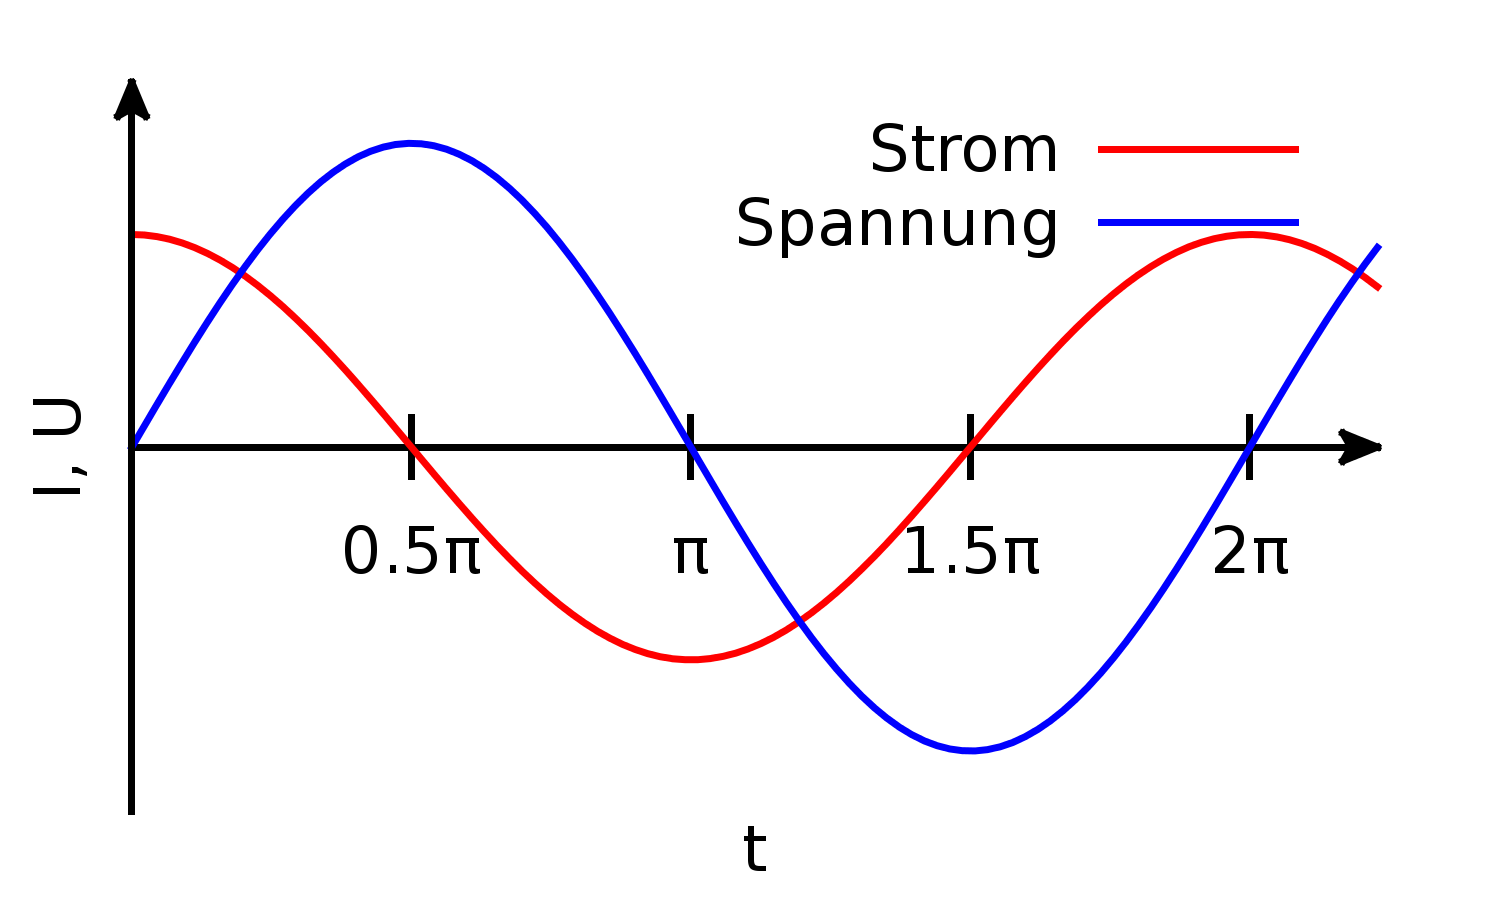
\includegraphics[width=0.7\textwidth]{plot_spannungen_vor_strom}
	\caption{\glqq Der Strom hinkt der Spannung um $\frac{\pi}{2}$ bzw. 90\degree{} hinterher.\grqq }
\end{figure}



\subsubsection{Impedanz}

Die Impedanz $Z$ ist der effektive Gesamtwiderstand im Wechselstromkreis. Die Impedanz trägt wie der Ohm'sche Widerstand die Einheit \emph{Ohm} mit Zeichen $\Omega$. Sie ist der Quotient aus der Spannung und der Stromstärke:

\begin{equation}		\label{eq:Impedanz}
	Z = \frac{U_{eff}}{I_{eff}}
	  = \frac{\hat{U}}{\hat{I}}
\end{equation}


\subsubsection{Kapazitiver Widerstand}

Für den kapazitiven Widerstand $X_C$, der von Kondensatoren im Wechselstromkreis ausgeht, siehe \referenz{subsec:KapazitiverWiderstand}.


\subsubsection{Induktiver Widerstand}

Für den induktiven Widerstand $X_L$, der von Spulen im Wechselstromkreis ausgeht, siehe \referenz{subsec:InduktiverWiderstand}.






